\section{\txnimp: Syntax and Semantics}
\label{sec:opsem}

\label{sec:syntax}

\renewcommand{\ctxn}[3]{\C{TXN}_{#1}\langle #2 \rangle\{#3\}}
\begin{figure*}[!ht]
\raggedright
%
\textbf{Syntax}\\
%
\begin{smathpar}
\renewcommand{\arraystretch}{1.2}
\begin{array}{lclcl}
\multicolumn{5}{c} {
  {x,y} \in \mathtt{Variables}\qquad
  {f} \in \mathtt{Field\;Names} \qquad
% {\tau} \in \mathtt{Table\;Names}
  {i,j} \in \mathbb{N} \qquad
  {\odot} \in \{+,-,\le,\ge,=\}\qquad
}\\
\multicolumn{5}{c}{
  {k} \in \mathbb{Z}\cup\mathbb{B} \qquad
  {\rec} \in \{\bar{f}=\bar{k}\}\qquad
  {\stl,\stg,s} \in \Pow{\rec} \qquad
  \I \in \mathbb{B}\times\Pow{\rec}\times\Pow{\rec}\times\Pow{\rec}
  \rightarrow \Prop
}\\
v & \in & \mathtt{Values} & \coloneqq & k \ALT \rec \ALT s\\
e & \in & \mathtt{Expressions} & \coloneqq & c \ALT x \ALT x.f 
    \ALT \{\bar{f}=\bar{e}\} \ALT e_1 \odot e_2\\ 
c & \in & \mathtt{Commands} & \coloneqq & \cskip \ALT \lete{x}{e}{c}
    \ALT \ite{e}{c_1}{c_2}\ALT c_1;c_2 \ALT \inserte{e}  \\
&&&&\ALT \deletee{\lambda x.e}
    \ALT \lete{x}{\selecte{\lambda x.e}}{c}
    \ALT \updatee{\lambda x.e_1}{\lambda x.e_2}\\
&&&&\ALT \foreache{e_1}{\lambda x.\lambda y. e_2} 
    \ALT \foreachr{s_1}{s_2}{\lambda x.\lambda y. e}\\
&&&&\ALT \ctxn{i}{\I}{ c } \ALT \ctxn{i}{\I,\stl,\stg}{c} \ALT c1 || c2\\
% t & \in & \mathtt{Terms} & \coloneqq & e \ALT c\\
\ectx & \in & \mathtt{Eval\;Ctx} & ::= & \bullet \ALT  
  \bullet || c_2 \ALT c_1 || \bullet \ALT \bullet;\,c_2 
  \ALT \ctxn{i}{\I,\stl,\stg}{\bullet} \\
\end{array}
\end{smathpar}
%
\bigskip

\renewcommand{\arraystretch}{1.2}

%
\textbf{Local Reduction} \quad 
\fbox {\(\stg \vdash (c,\stl) \stepsto (c',\stl')\)}\\
%
\begin{minipage}{2.8in}
\rulelabel{E-Insert}
\begin{smathpar}
\begin{array}{c}
\RULE
{
  i \not\in \dom(\stl \cup \stg)\\
  r = \{\bar{f}=\bar{k};\,\idf=i;\,\delf=\C{false}\}
}
{
  \stg \vdash (\inserte{\{\bar{f}=\bar{k}\}},\stl) \stepsto
  (\cskip,\stl \cup \{r\})
}
\end{array}
\end{smathpar}
\end{minipage}
%
%
\begin{minipage}{2.8in}
\rulelabel{E-Delete}
\begin{smathpar}
\begin{array}{c}
\RULE
{
  s = \{r' \,|\, \exists(r\in\Delta).~ \eval([r/x]e)=\C{true} \\
        \hspace*{0.7in}\conj r'=\{\bar{f}=r.\bar{f}; \idf=r.\idf;
        \delf=\C{true}\}\}\\
% \dom(s) \cap \dom(\delta) = \emptyset
}
{
  \stg \vdash (\deletee{\lambda x.e},\stl) \stepsto (\cskip,\stl \cup s)
}
\end{array}
\end{smathpar}
\end{minipage}
%
\bigskip

%
\begin{minipage}{2.8in}
\rulelabel{E-Select}
\begin{smathpar}
\begin{array}{c}
\RULE
{
  s = \{r\in\Delta \,|\, \eval([r/x]e)=\C{true}\}\spc
  c' = [s/x]c
}
{
  \stg \vdash (\lete{x}{\selecte{\lambda x.e}}{c}, \stl) \stepsto 
              (c',\stl)
}
\end{array}
\end{smathpar}
\end{minipage}
%
%
\begin{minipage}{2.8in}
\rulelabel{E-Update}
\begin{smathpar}
\begin{array}{c}
\RULE
{
  s = \{r' \,|\, \exists(r\in\Delta).~ \eval([r/x]e_2)=\C{true} \conj r'=[r/x]e_1\}\\
}
{
  \stg \vdash (\updatee{\lambda x.e_1}{\lambda x.e_2},\stl) \stepsto 
              (\cskip,\stl \cup s)
}
\end{array}
\end{smathpar}
\end{minipage}
%

\begin{smathpar}
\begin{array}{ll}
  \rulelabel{E-Foreach1} & \stg \vdash (\foreache{e}{\lambda x.\lambda
  y.c},\stl) \stepsto (\foreachr{\emptyset}{\eval(e)}{\lambda x.\lambda y. c})\\
  \rulelabel{E-Foreach2} & \stg \vdash (\foreachr{s_1}{\{r\} \cup s_2}{\lambda x.\lambda
  y.c},\stl) \stepsto ([r/y][s_1/x]c;\,\foreachr{s_1 \cup \{r\}}{s_2}{\lambda x.\lambda y. c})\\
  \rulelabel{E-Foreach3} & \stg \vdash (\foreachr{s}{\emptyset}{\lambda x.\lambda
  y.c},\stl) \stepsto (\cskip,\stl)\\
\end{array}
\end{smathpar}
%
\bigskip

%
\textbf{Top-Level Reduction} \quad 
\fbox {\((c,\stg) \stepsto (c',\stg')\)}\\
%
\begin{minipage}{3in}
\rulelabel{E-Txn}
\begin{smathpar}
\begin{array}{c}
\RULE
{
  \I(\C{true},\stl,\stg,\stg')\spc
  \stg \vdash (c,\stl) \stepsto (c',\stl')
}
{
  (\ctxn{i}{\I,\stl,\stg}{c},\stg') \stepsto
  (\ctxn{i}{\I,\stl',\stg'}{c'},\stg')
}
\end{array}
\end{smathpar}
\end{minipage}
%
%
\begin{minipage}{2.8in}
\rulelabel{E-Commit}
\begin{smathpar}
\begin{array}{c}
\RULE
{
  \I(\C{false},\stl,\stg,\stg')
}
{
  (\ctxn{i}{\I,\stl,\stg}{\cskip},\stg') \stepsto (\cskip,\stl\gg\stg')
}
\end{array}
\end{smathpar}
\end{minipage}
%


\caption{\small \txnimp: Syntax and Small-step semantics}
\label{fig:txnimp}
\end{figure*}



Fig.~\ref{fig:txnimp} shows the syntax and small-step semantics of
\txnimp, a core language that we will use to formalize the intuitions
presented in the previous section. Natural numbers, (shared) variables
and arithmetic expressions constitute the syntactic class of
expressions ($e$).  Commands ($c$) include $\cskip$, assignment
statements, transaction (\C{txn}) lexical blocks, and their sequential
and parallel composition. We let $T_i$ for $i \in \mathbb{N}$ range
over transaction identifiers. When it is evident we are referring to a
transaction, we use the number $i$ instead of $T_i$ for identification
(\eg, in $\C{txn}\langle i \rangle$). For notational convenience, we
let $t$ range over both expressions and commands.

We define a small-step operational semantics for this language in
terms of an abstract machine that generates an execution trace
($\E$). The first component of the trace is a set ($\A$) of
\emph{effects}, where an effect ($\eta$) documents a read (\C{RD(X)}),
a write (\C{WR(X)}), or a transaction commit (\C{COMMIT}) operation
performed during the execution. Any value associated with the
operation (\eg, value read or value written) is also documented, and
can be accessed via $\rval$. Every effect has a unique identifier
accessible via $\id$, and a transaction identifier accessible via
$\txn$.  The latter identifies the transaction that generated the
effect. In every step of the evaluation, the machine reduces a \txnimp\
term by executing a read, write or commit operation, generating an
effect, and extending the trace. Since effects include transaction
identifiers, the semantics distinguishes between terms ($t$) of
different transactions. For example, $\txnbox{t}_i$ denotes a term $t$
inside a transaction $T_i$.  Evaluation contexts are also
appropriately marked. For example, $\ectx_i$ denotes the evaluation
context for a term inside $T_i$. The other component of an execution
trace is a visibility relation ($\visZ$) that establishes a visibility
property between effects among different transactions. The intent and
mechanics of $\visZ$ is described in the sequel.

Fundamental to our development is the notion of a trace invariant
($\I$). $\I$ is a function from traces ($\E$) to first-order logical
formula ($\Prop$) that define well-formedness
constraints over traces.  The machine takes a step only if the
resulting trace satisfies the constraints imposed by $\I$. This
behavior is captured by the auxiliary reduction rule
\rulelabel{E-Aux} that factors out the trace extension aspect of the
evaluation by abstracting away the operation-specific behavior as a
function that generates an appropriate effect. We let $\mathcal{F}$
denote this function.  \rulelabel{E-Aux} uses $\mathcal{F}$ to
generate a new effect and extend the trace ($\E = (\A,\visZ)$)
\emph{only if} the well-formedness constraints imposed by $\I$ on $\E$
(i.e., $\I(\E')$) are satisfied. Otherwise, it gets stuck. In an
execution that runs to completion, every small-step preserves the
well-formedness of a trace, thus ensuring the invariance of $\I$.
Note that the semantics makes no assumptions about $\I$ other than its
type. As such, it can be instantiated with any trace-parametric
proposition that expresses constraints over the given trace. For
instance, consider the $\psi_{RC}$ specification from
\S\ref{sec:motivation}, but with bounded $T_1$ and $T_2$ instantiated
with \C{Wd1} and \C{Wd2}, respectively. The instantiated specification
is the following term:

\begin{smathpar}
\begin{array}{l}
  \forall \eta_1,\eta_2,.\; \txn(\eta_1) = \C{Wd1}
  \conj \txn(\eta_2) = \C{Wd2} \\
  \hspace*{0.6in}\conj \C{Wd1} \neq \C{Wd2} \conj \eta_1 \hboar
  \eta_2 \Rightarrow \C{Wd1} \hboar \eta_2 \\
\end{array}
\end{smathpar}

\noindent It is easy to interpret the above specification in the
context of a trace $\E$ that captures an execution of the program in
Fig.~\ref{fig:motiv-eg-1}. Such a trace-parametric formula can be
used to instantiate the trace invariant $\I$ in Fig.~\ref{fig:txnimp}.
The resultant operational semantics describes an abstract machine that
gets stuck if an operation of \C{Wd2} is executed in a state that
incorporates some, but not all the effects (including the \C{COMMIT})
of \C{Wd1}.
% While the machine takes a step only if the constraints are
% satisfied, it neither defines nor explicitly assumes an oracle to
% check satisfaction.

As described in \S\ref{sec:motivation}, the semantics of various
isolation levels can be captured as constraints over the
happens-before ($\hbZ$) relation. $\hbZ$ is however a derived relation
in our model, composed of more fundamental \emph{session order}
($\soZ$) and \emph{visibility} ($\visZ$) relations, which shall
henceforth replace $\hbZ$ in the discussion.  A session order relation
captures the sequential order of operations within a transaction. In
particular, it relates two effects, $\eta_1$ and $\eta_2$, such that
$\txn(\eta_1) = \txn(\eta_2)$ and $\id(\eta_1) < \id(\eta_2)$.  The
semantics assigns monotonically increasing identifiers to effects, as
defined by the $\id(\eta) > \maxId(\A)$ condition of
\rulelabel{E-Aux}.  Evaluation contexts ($\ectx_i$) for
transaction-bound terms are defined so as to enforce a deterministic
sequential order of execution within a transaction, leading to a
deterministic total order among effect ids, which defines the session
order relation. Visibility ($\visZ$) on the other hand relates effects
across concurrent transactions.  Intuitively, $\visZ$ relates $\eta_1$
to $\eta_2$ if and only if $\eta_1$ was \emph{visible} to the
operation that generated $\eta_2$ during its execution, thus effecting
its return value ($\rval(\eta_2)$). For example, a read operation over
\C{X} may pick the value ($\rval$) of the write effect with the highest id
among its visible effects (this is made possible by appropriately
defining $\interp{\cdot}$ in \rulelabel{E-Var}, as we show later).
Thus, the value of a read depends on what write effects it can
witness. An operation can only witness the effects of already
concluded operations, which varies between executions due to the
non-deterministic order of evaluating the parallel composition of
transactions.

A more notable source of non-determinism, however, is the
\rulelabel{E-Aux} rule, which allows the machine to expose an
arbitrary subset ($S$) of existing effects ($\A$) to the incoming
operation. In other words, the machine is not obligated to reveal the
effects of all previous operations to an incoming operation. This
relaxation allows the abstract machine to model the semantics of
weakly-consistent data stores. For instance, operations issued to an
eventually consistent ({\sc ec}) replicated store could be dispatched
to different replicas whose states may not be in any well-defined
relationship. By allowing operations to witness arbitrary subsets of
the global state, the semantics models the weak visibility properties
of such stores; we elaborate on the implication of this style of
definition in \S\ref{sec:store-consistency}.  Stronger visibility
properties can be expressed by imposing well-formedness constraints
over $\visZ$ via the trace invariant ($\I$). Since the abstract
machine is obligated to satisfy $\I$ at every step of the execution,
operations are guaranteed to experience the level of isolation
specified by $\I$.  Thus, in executions that run to completion, the
abstract machine models a store that provides the required levels of
isolation.  Notably, the machine achieves this without defining an
operational semantics for isolation levels, instead solely relying on
their declarative characterization as trace well-formedness
constraints to enforce isolation guarantees.
\S\ref{sec:ansi-isolation} shows the specification of various ANSI SQL
isolation levels stated as trace well-formedness constraints.

% TRACE RELATIONS
% ---------------
\begin{figure*}[t!]
\begin{minipage}{\columnwidth}
\begin{smathpar}
\begin{array}{lcl}
(\A,\visZ) \Vdash \eta \in T_i & \defeq & \eta \in \A \conj \txn(\eta) = T_i\\
\E \Vdash S \subseteq T_i & \defeq & \forall \eta.~ \eta
        \in S \Rightarrow \underE{\eta \in T_i} \\
(\A,\visZ) \Vdash \eta_1 \visar \eta_2 & \defeq & \{\eta_1,\eta_2\}
        \subseteq \A \conj (\eta_1,\eta_2) \in \visZ\\
(\A,\visZ) \Vdash \eta_1 \soar \eta_2 & \defeq & \{\eta_1,\eta_2\}
        \subseteq \A \conj \txn(\eta_1)=\txn(\eta_2) \\
        &   & \hspace*{0.3in} \conj \id(\eta_1) < \id(\eta_2)\\
\E \Vdash T_i \visar \eta & \defeq &\forall\eta_1
        .\,(\E \Vdash \eta_1 \in T_i) \Rightarrow \E \Vdash \eta_1 \visar \eta \\
\end{array}
\end{smathpar}
\end{minipage}
\begin{minipage}{\columnwidth}
\begin{smathpar}
\begin{array}{lcl}
\underE{T_i \visar T_j} & \defeq &  \forall\eta_1,\eta_2.\,
    %\sameobj{\eta_1}{\eta_2}  \Rightarrow 
    \underE{\eta_1\in T_i} \conj \underE{\eta_2 \in T_j} \\
    &   & \hspace*{1in}\Rightarrow \underE{\eta_1 \visar \eta_2} \\
\underE{T_i \invisar T_j} & \defeq &  \forall\eta_1,\eta_2.\,
        %\sameobj{\eta_1}{\eta_2}\Rightarrow 
        \underE{\eta_1\in T_i} \conj \underE{\eta_2 \in T_j}\\
    &   & \hspace*{1in} \Rightarrow \neg (\underE{\eta_1 \visar \eta_2})\\
\underE{T_i \wrstoar X} & \defeq & \exists\eta.~
        \underE{\eta \in T_i} \conj \kind(\eta) = \C{WR}(X)\\
\underE{T_i \rdsfmar X} & \defeq & \exists\eta.~
        \underE{\eta \in T_i} \conj \kind(\eta) = \C{RD}(X)\\
\underE{T_i \usesar X} & \defeq & \underE{T_i \wrstoar X} \disj
      \underE{T_i \rdsfmar X}\\
\end{array}
\end{smathpar}
\end{minipage}

\caption{Relations defined over a trace}
\label{fig:rel-defs}
\end{figure*}




% However, a machine that lets operations witness arbitrary subset of
% the global state offers no isolation whatsoever. For example, it may
% allow a read operation to witness writes of an uncommitted
% transaction, violating RC isolation. Fortunately, our ability to
% express an isolation semantics as constraints over happens-before
% order through $\visZ$ and $\soZ$ relations, and the property of the
% abstract machine to be parametric over the trace invariant ($\I$),
% lets us solve this problem.
% In particular, we continue to define isolation semantics as
% constraints over $\visZ$ and $\soZ$, but confine their domain of
% interpretation to the given trace so that they now become trace
% well-formedness constraints. Well-formedness constraints can be
% combined into a trace invariant ($\I$). 


As described previously, \rulelabel{E-Aux} abstracts away the
operation-specific behavior of a machine step as a function ($\F$)
that accepts a set ($S$) of effects chosen by the machine to make
visible to the operation, interprets the operation w.r.t. $S$, and
returns an appropriate effect that encodes its return value. Rules
\rulelabel{E-Var}, \rulelabel{E-Asgn} and \rulelabel{E-Commit} define
such functions for read, write and commit operations, respectively.
The effect returned by the function in each case includes its
transaction id ($T_i$) along with an arbitrarily chosen effect id
($j$) that is later verified to be unique in \rulelabel{E-Aux}. The
$\rval$ for a write is the value being written, and for commit it is
$\bot$. In case of a read, the value read depends on how the read
operation chooses to interpret the given set ($S$) of visible effects.
The interpretation may depend on application semantics. For example, a
monotonically increasing counter application may choose to let a write
with the largest value determine the value of a read. To accommodate
multiple interpretations, the semantics is made parametric over an
interpretation function ($\interp{\cdot}$) that accepts a set of
effects and a variable name, and returns the value associated with the
variable. A straightforward interpretation function that chooses the
last write (i.e., write with largest id) is shown below:

\begin{smathpar}
\begin{array}{lcl}
  \isMax(S,\eta) & \Leftrightarrow &  \forall (\eta'\in S).  
  \kind(\eta') = \kind(\eta) \\
  & & \hspace*{0.4in}\Rightarrow \eta' = \eta \disj \id(\eta') < \id(\eta)\\

\interp{S}(X) & = & \C{if}\;(\exists (\eta \in S). \kind(\eta) = \C{WR}(X) 
  \wedge \isMax(S,\eta)) \\
  & & \C{then}\;\rval(\eta)\;\C{else}\;0\\
\end{array}
\end{smathpar}

\noindent Rules \rulelabel{E-Top-Ctx} and \rulelabel{E-Txn-Ctx} define
congruence properties for top-level terms and transaction-bound terms,
respectively. The rules and evaluation contexts ($\ectx$ and
$\ectx_i$) are defined such that only certain kinds of terms are
allowed at the top-level and inside a transaction. In particular, a
\txnimp program at the top-level can either be a transaction, or a
parallel composition of transactions. A command inside a \C{txn} block
can either be an assignment, or a sequential composition of
assignments. 

\subsection{Specifications}
\label{sec:ansi-isolation}


% ISOLATION SPECS
% ---------------
\begin{figure*}[t!]
\begin{smathpar}
\begin{array}{lcl}
\underE{\C{RMWVis}(T_j)} & \defeq & \forall\eta_1,\eta_2.\,
       \underE{\{\eta_1,\eta_2\} \subseteq T_j} \conj
       \underE{\eta_1 \soar \eta_2} \Rightarrow \underE{\eta_1 \visar
       \eta_2}\\
\underE{\C{MonotonicVis}(T_j)} & \defeq & 
       \underE{\C{RMWVis}(T_j)} \conj 
       \forall\eta,\eta_1,\eta_2.\, \underE{\{\eta_1,\eta_2\} \in T_j} 
          \conj \\
  &   & \hspace*{1.2in}\underE{\eta \visar \eta_1} \conj
        \underE{\eta_1 \soar \eta_2} \Rightarrow \underE{\eta \visar
        \eta_2} \\
%  \C{CausalVis}(T_i) & \defeq & 
%         \C{MonotonicVis}(T_i) \conj \C{RMWVis}(T_i)\\
\underE{\C{AtomicVis}(T_j)} & \defeq & 
       \forall\eta_1,\eta_2.\, \neg(\underE{\eta_1 \in T_j}) \conj
       \underE{\eta_2 \in T_j} \conj
       \underE{\eta_1 \visar \eta_2} \Rightarrow \underE{\txn(\eta_1)
       \visar \eta_2}\\
\underE{\C{CommitVis}(T_j)} & \defeq & 
       \forall\eta_1,\eta_2.~ \neg(\underE{\eta_1 \in T_j}) \conj 
          \underE{\eta_2 \in T_j} \conj
       \underE{\eta_1 \visar \eta_2} \Rightarrow\\
  &   & \hspace*{1.2in}\exists\eta.\, \underE{\eta \in \txn(\eta_1)} 
        \conj \kind(\eta) = \C{COMMIT} 
        \conj \underE{\eta \visar \eta_2}\\
% \underE{\C{TransVis}(T_j)} & \defeq &  \forall
%        \eta_1,\eta_2,\eta_3.\, \underE{\eta_3 \in T_j} \conj
%        \underE{\eta_1 \visar \eta_2} \conj
%        \underE{\eta_2 \visar \eta_3} \Rightarrow \underE{\eta_1 \visar
%        \eta_3} \\
\underE{\C{RC}(T_j)} & \defeq & \underE{\C{AtomicVis}(T_j)} 
        \conj \underE{\C{CommitVis}(T_j)}\\
\underE{\C{MAV}(T_j)} & \defeq & \underE{\C{RC}(T_j)} \conj
      \underE{\C{MonotonicVis}(T_j)} \\
\underE{\C{SnapshotVis}(T_i,T_j)} & \defeq &  \underE{T_i
       \visar T_j} \disj \underE{T_i \invisar T_j}\\
\underE{\C{RR}(T_j)} & \defeq & \underE{\C{MAV}(T_j)}
       \conj \forall T_i.\,T_i \neq T_j \Rightarrow 
        \underE{\C{SnapshotVis}(T_i,T_j)} \\
% &   & \hspace*{2in}\conj  \C{SnapshotVis}(T_i,T_j)\\
\underE{\C{SnapshotSER}(T_i,T_j,X)} & \defeq &  \underE{T_i
       \visar T_j} \disj (\underE{T_i \invisar T_j} \conj \\
  &   &\hspace*{1.2in}\exists \eta.~\underE{\eta\in T_i} \conj \kind(\eta) =
       \C{WR(X)} \Rightarrow \underE{T_j \visar \eta})\\
\underE{\C{SI}(T_j)} & \defeq &  \underE{\C{RR}(T_j)}
       \conj \forall T_i.\,(T_i \neq T_j \conj \exists X.\, \underE{T_i \wrstoar X} \conj 
        \underE{T_j \wrstoar X})\\
%      (\exists X.\, T_i \wrstoar X \conj T_j \wrstoar X)
%      \Rightarrow  \C{TotalVis}(T_i,T_j)\\
  &   & \hspace*{2in} \Rightarrow \underE{\C{SnapshotSER}(T_i,T_j,X)}\\
\underE{\C{SER}(T_j)} & \defeq & \underE{\C{RR}(T_j)}
        \conj \forall T_i.\,(T_i \neq T_j \conj \exists X.\, 
        \underE{T_i \wrstoar X} \conj \underE{T_j \usesar X})\\
  &   & \hspace*{2in} \Rightarrow \underE{\C{SnapshotSER}(T_i,T_j,X)}\\
\end{array}
\end{smathpar}

\caption{Standard isolation guarantees expressed as trace
well-formedness constraints}
\label{fig:ansi-isolation}
\end{figure*}




We now describe specifications of standard isolation guarantees
expressed as constraints over trace well-formedness. For brevity and
convenience, we introduce some notations that are used in the following
sections.  An execution trace is destructed as ($\A$,$\visZ$) whenever
individual components of the pair are needed. Otherwise, it is written
as $\E$.  Sometimes, the dot notation (\eg~$\E.\A$) is also
used. Since $\A$ and $\visZ$ are both sets, we lift the operations on
sets to pairs of sets when updating $\E$. For example, $\E' = \E \cup
(\{\eta_2\},\{(\eta_1,\eta_2)\})$ expands to $\E' = (\E.\A \cup
\{\eta_2\},\,\E.\visZ \cup \{(\eta_1,\eta_2)\})$.  When $\psi$ is a
formula, $\underE{\psi}$ denotes the interpretation of $\psi$ in the
context of the trace $\E$. Such interpretations are defined on a
case-by-case basis in Figs.~\ref{fig:rel-defs}
and~\ref{fig:ansi-isolation}.

\subsubsection{Trace Relations}

Fig.~\ref{fig:rel-defs} shows various relations defined over elements
in a trace. In the context of a trace $(\A,\visZ)$, an effect $\eta$
is said to belong to a transaction $T_i$ if $\eta$ belongs to the
effect set $A$ and its transaction identifier is $T_i$. The
containment relation is trivially lifted to the set of effects to
define $\underE{S \subseteq T_i}$.  Visibility, session order, and
happens-before relations are denoted by $\eta_1 \visar \eta_2$,
$\eta_1 \soar \eta_2$, and $\eta_1 \hboar \eta_2$, respectively. A
transaction $T_i$ is said to be visible to an effect $\eta$ if every
effect $\eta_1$ of $T_i$ recorded by the trace is visible to $\eta$.
$T_i$ may be visible to $\eta$ but may not be visible to every other
effect in the $\txn(\eta)$. For a transaction $T_i$ to be considered
to be visible to a transaction $T_j$ in the context of a trace $\E$
(written $\underE{T_i \visar T_j}$), every effect ($\eta_1$) of $T_i$
present in $\E$ must be visible to every effect ($\eta_2$) of $T_j$ in
$\E$.  Conversely, if none of the effects of $T_i$ present in $\E$ are
visible to any effect of $T_j$, then $T_i$ is considered invisible to
$T_j$ under $\E$ (written $\underE{T_i \invisar T_j}$). Transaction
$T_i$ is said to have written to a variable $X$ under $\E$ (i.e.,
$\underE{T_i \wrstoar X}$) if there exists a $\C{WR}(X)$ effect from
$T_i$ in $\E$.  \emph{Reads-from} ($\underE{T_i \rdsfmar X}$) is
defined similarly. $T_i$ \emph{uses} $X$ ($T_i \usesar X$) if it reads
or writes $X$.

Fig.~\ref{fig:ansi-isolation} shows various isolation guarantees
defined as propositions indexed by transaction identifiers.
Transaction $T_j$ is said to have experienced \emph{read-my-writes}
visibility under $\E$ if every effect ($\eta_1$) of $T_j$ is visible
to every subsequent effect ($\eta_2$) of the same transaction in $\E$.
This lets $T_j$ to never lose its own updates. Monotonic visibility
adds one more constraint to \emph{read-my-writes}; besides requiring $\eta_1$
to be visible to $\eta_2$, it also requires every effect ($\eta$)
visible to $\eta_1$ in $\E$ to be visible to $\eta_2$ as well. Thus,
later operations in a transaction witness at least the same set of
effects witnessed by the earlier operations, if not more (hence,
``monotonic'' visibility). Atomic visibility allows an effect
$\eta_2$ of $T_j$ to witness an effect $\eta_1$ of $T_i$ only if all
effects of $T_i$ in $\E$ are also visible to $\eta_2$. Atomic
visibility thus prevents a transaction from being partially visible.
However, atomic visibility does not prevent an uncommitted transaction
from being visible. This is addressed by \C{CommitVis}, which requires
the commit effect of $T_i$ to be visible whenever any effect of $T_i$
is visible.

\subsubsection{Isolation Levels}

Fig.~\ref{fig:ansi-isolation} shows specifications of various
well-known isolation guarantees.  The ANSI SQL 92 standard requires
\iso{Read Committed} isolation to avoid the dirty reads phenomenon,
which is achieved by enforcing $\mathtt{AtomicVis}$ and
$\mathtt{CommitVis}$ guarantees. The {\sc rc} specification
(\C{RC})\footnote{In the following, we use small caps to abbreviate
isolation levels (\emph{e.g.,} {\sc rc} for \emph{Read Committed}),
and typewriter font for abbreviations of the specification of an
isolation level (\emph{e.g.,} \C{RC} denotes the specification for
{\sc rc} as given in Fig.~\ref{fig:ansi-isolation}).} is therefore a
combination of these two guarantees. The specification also agrees
with the description and implementation~\cite{bailishat,pldi15} of
{\sc rc} for highly available replicated stores. On relational
databases, however, {\sc rc} has also come to be associated with the
$\mathtt{MonotonicVis}$ guarantee.  Nonetheless, $\mathtt{AtomicVis}$
and $\mathtt{CommitVis}$ are sufficient to reason about {\sc rc}
isolation on relational stores too. The combination of these
guarantees with the {\sc sc} property of relational stores (formalized
in \S\ref{sec:store-consistency}) automatically leads to the
monotonicity guarantee, which explains why {\sc rc} comes with
$\mathtt{MonotonicVis}$ on such stores regardless of the
implementation. On weakly consistent stores however,
$\mathtt{AtomicVis}$ and $\mathtt{CommitVis}$ do not imply
$\mathtt{MonotonicVis}$. A stronger isolation level called
\iso{Monotonic Atomic View} ({\sc mav} of
Fig.~\ref{fig:ansi-isolation})~\cite{bailishat} was proposed to
explicitly extend {\sc rc} with monotonicity on such stores. 


Snapshot visibility (\C{SnapshotVis}) captures the scenario where a
transaction executes against a static snapshot of the database.  A
transaction $T_i$ is said to be snapshot-visible to a transaction
$T_j$ if either it is visible to $T_j$ (i.e., $T_i$ is included in the
snapshot), or it is invisible (i.e., it is not included); it is
forbidden for only a suffix (more generally, a subset) of $T_j$ to
witness $T_i$. The specification of ANSI SQL \iso{Repeatable Read}
isolation (\C{RR}) extends \C{MAV} with the snapshot visibility
guarantee.  Observe that snapshot visibility permits $T_i$ and $T_j$
to execute and commit while being oblivious of each other. This
scenario is captured in Fig.~\ref{fig:ansi-iso-eg-rr}, where
transactions $T_1$ and $T_2$, which perform conflicting writes,
execute against a snapshot of the database and commit concurrently.
While the actual values read and written by $T_1$ and $T_2$ are
unimportant (hence, elided), it is important to note the
\emph{absence} of visiblity arrows from $T_2$ to $T_1$, although $T_2$
commits before $T_1$'s read-from-$Y$.

\iso{Snapshot Isolation} ({\sc si}) proscribes this possibility. If
$T_i$ and $T_j$ both write to the same shared variable, then {\sc si}
insists that either $T_i$ be visible to $T_j$, or $T_j$ be visible to
the conflicting write of $T_i$ (this is captured by the auxiliary
definition \C{SnapshotSER}). Fig.~\ref{fig:ansi-iso-eg-si} shows an
execution where {\sc si} transaction $T_1$ witnesses a snapshot of the
database that doesn't include $T_2$. Due to \C{SI($T_1$)}, the
conflicting write to $X$ in $T_2$ is now required to witness $T_1$, as
captured by the direction of the $\visZ$ arrow (subsequent operations
also witness $T_1$ because $T_2$ is executing under {\sc mav}).
Lastly, \iso{Serializable} isolation extends $\mathtt{SnapshotSER}$ to
also cover non-conflicting transactions that write to variables read
in the current transaction.  Fig.~\ref{fig:ansi-iso-eg-ser} shows an
execution of an {\sc ser} transaction $T_3$ and a {\sc mav}
transaction $T_4$, which write to $X$ and $Y$, respectively. The
snapshot witnessed by the {\sc ser} transaction $T_3$ does not include
$T_4$, but the write to $Y$ in $T_4$, although non-conflicting,
witnesses $T_1$ because $Y$ is read by $T_1$. Visibility includes
other operations of $T_4$ because of {\sc mav}. Note that {\sc ser}
does not guarantee a total order on transactions w.r.t. $\visZ$
because, in practice, databases do not guarantee global serializable
execution unless \emph{all} transactions choose {\sc ser}.

\begin{figure}
\centering
\subcaptionbox {
  {\sc rr}($T_1$), {\sc rr}($T_2$).
  \label{fig:ansi-iso-eg-rr}
} [
  0.33\columnwidth
] {
  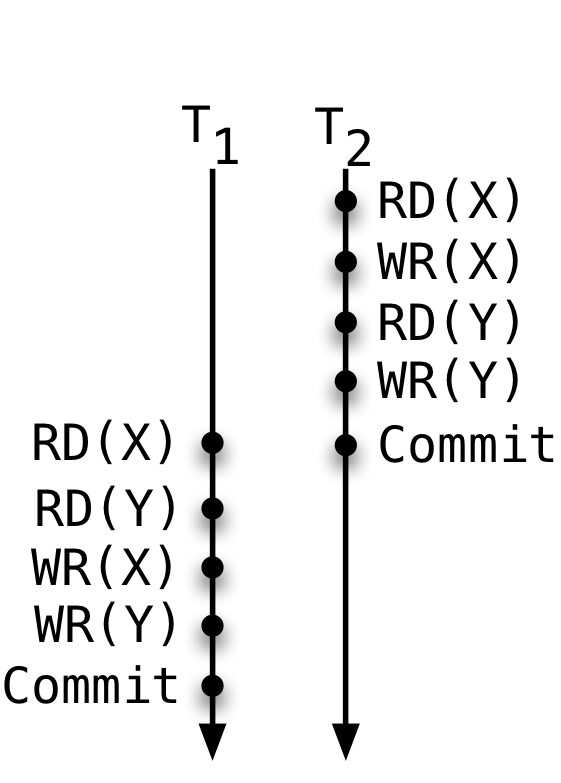
\includegraphics[scale=0.36]{Figures/rr-eg}
}
\subcaptionbox {
  {\sc si}($T_1$), {\sc mav}($T_2$)
  \label{fig:ansi-iso-eg-si}
} [
  0.33\columnwidth
] {
  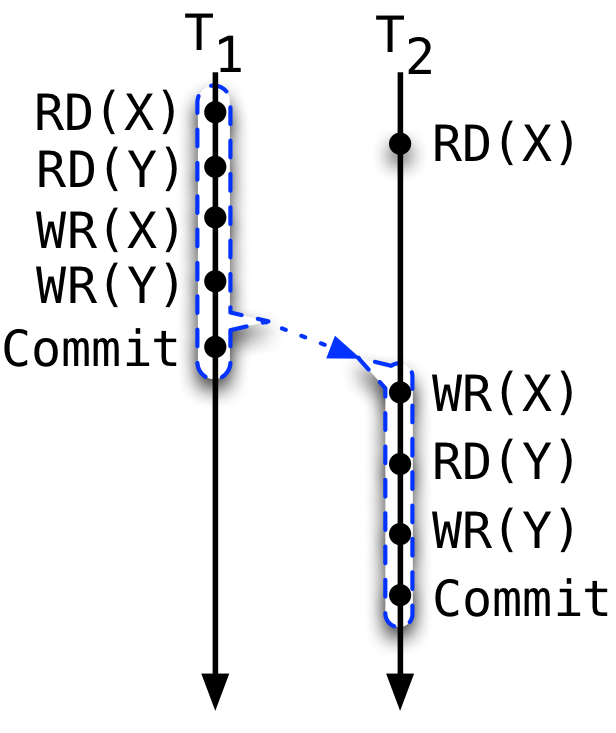
\includegraphics[scale=0.36]{Figures/si-eg-2}
}
\subcaptionbox {
  {\sc ser}($T_3$), {\sc mav}($T_4$)
  \label{fig:ansi-iso-eg-ser}
}{
  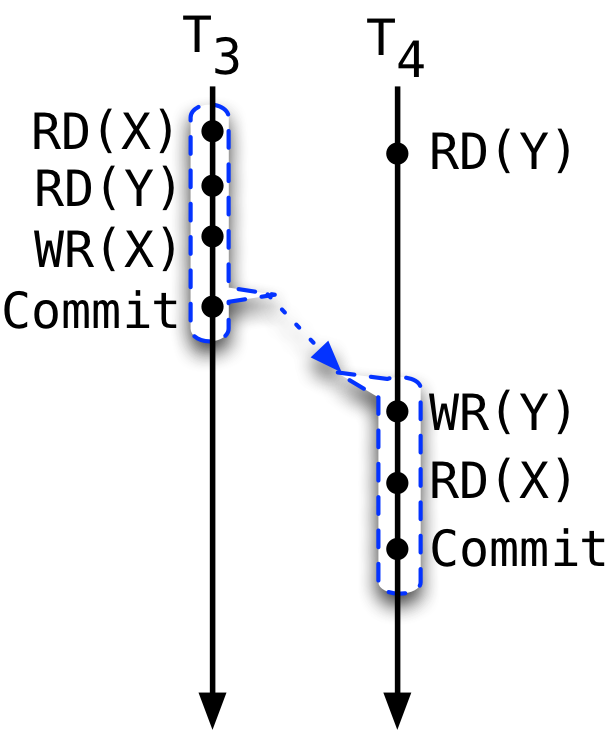
\includegraphics[scale=0.32]{Figures/ser-eg}
}

\caption{\small Sample executions of concurrent transactions at different
isolation levels. Solid (black) arrows indicate the timeline. Points
on the timeline mark the time when an operation is executed. Dotted
(blue) arrows denote $\visZ$. }
\label{fig:ansi-iso-eg}
\vspace*{-12pt}
\end{figure}

% Note that both $\mathtt{SnapshotVis}$ and $\mathtt{OneWaySER}$
% are asymmetric definitions that guarantee complete visiblity or
% invisibility of $T_i$ to $T_j$, but not the converse. While
% $\mathtt{SnapshotVis}$ provides no guarantees to $T_i$,
% $\mathtt{OneWaySER}$ guarantees that at least the commit effect of
% $T_i$ witnesses $T_j$. 

% \iso{Snapshot Isolation} spec ({\sc si}) extends {\sc rr} with a
% one-way serializability guarantee w.r.t. the transactions that perform
% conflicting writes (i.e., writes to the same shared variable).
% \footnote{Fig.~\ref{fig:ansi-isolation} presents slightly
% weaker versions of {\sc si} and {\sc ser} specs in the interest of
% clarity.}. Fig.~\ref{fig:ansi-iso-eg} shows sample executions of
% transactions $T_1$ and $T_2$. Both transactions read and write to
% shared variables $X$ and $Y$. In the first execution, $T_2$ commits
% while $T_1$ is still in progress, but {\sc rr} isolation prevents
% $T_1$ from witnessing the writes of $T_2$. In the second execution,

%% SJ: Not sure this paragraph is necessary here.
%% In contrast to recent proposals (\emph{e.g.},
%% ~\cite{gotsmanconcur15}), our specifications for {\sc si} and {\sc
%%   ser} do not necessarily impose a total order among transactions
%% (conflicting or otherwise). In reality, a total order under {\sc ser}
%% (resp. {\sc si}) is guaranteed only if the store executes all
%% transactions under {\sc ser} (resp. {\sc si}) isolation. Our
%% specifications admit this possibility, and derive a total order under
%% the assumption of homogenity. However, databases almost always allow
%% isolation levels to be configured on a per-transaction basis, allowing
%% transactions at various isolation levels to coexist.  Specifications
%% that assume homogenity are incorrect under this setting.

% Having specified isolation levels as trace well-formedness
% constraints, we can now construct trace invariants ($\I$) for
% \txnimp programs by composing isolation specifications for various
% transactions. For instance, the following trace invariant enforces
% {\sc si} for both transactions of the program in
% Fig.~\ref{fig:motiv-eg-1}, allowing it to satisfy its postcondition:
% \begin{smathpar}
% \I \;=\; \lambda\E.~ \underE{\C{SI(Wd1)}} \conj \underE{\C{SI(Wd2)}}
% \end{smathpar}
% In contrast, the following trace invariant enforces {\sc rc} for one and {\sc si}
% for another, leading to a possible violation of the postcondition:
% \begin{smathpar}
% \I \;=\; \lambda\E.~ \underE{\C{RC(Wd1)}} \conj \underE{\C{SI(Wd2)}}
% \end{smathpar}


